\let\negmedspace\undefined
\let\negthickspace\undefined
\documentclass[journal]{IEEEtran}
\usepackage[a5paper, margin=10mm, onecolumn]{geometry}
%\usepackage{lmodern} % Ensure lmodern is loaded for pdflatex
\usepackage{tfrupee} % Include tfrupee package

\setlength{\headheight}{1cm} % Set the height of the header box
\setlength{\headsep}{0mm}     % Set the distance between the header box and the top of the text

\usepackage{gvv-book}
\usepackage{gvv}
\usepackage{cite}
\usepackage{amsmath,amssymb,amsfonts,amsthm}
\usepackage{algorithmic}
\usepackage{graphicx}
\usepackage{textcomp}
\usepackage{xcolor}
\usepackage{txfonts}
\usepackage{listings}
\usepackage{enumitem}
\usepackage{mathtools}
\usepackage{gensymb}
\usepackage{comment}
\usepackage[breaklinks=true]{hyperref}
\usepackage{tkz-euclide} 
\usepackage{listings}
% \usepackage{gvv}                                        
\def\inputGnumericTable{}                                 
\usepackage[latin1]{inputenc}                                
\usepackage{color}                                            
\usepackage{array}                                            
\usepackage{longtable}                                       
\usepackage{calc}                                             
\usepackage{multirow}                                         
\usepackage{hhline}                                           
\usepackage{ifthen}                                           
\usepackage{lscape}
\begin{document}

\bibliographystyle{IEEEtran}
\vspace{3cm}

\title{NCERT-9.5.17.2}
\author{EE24BTECH11065 - Spoorthi yellamanchali}
% \maketitle
% \newpage
% \bigskip
{\let\newpage\relax\maketitle}

\renewcommand{\thefigure}{\theenumi}
\renewcommand{\thetable}{\theenumi}
\setlength{\intextsep}{10pt} % Space between text and floats


\numberwithin{equation}{enumi}
\numberwithin{figure}{enumi}
\renewcommand{\thetable}{\theenumi}


\textbf{Question:}
\\
Find the solution of the following differential equation:
\begin{align*} 
 xy\brak{dx} = \brak{x^3 + y^3}\brak{dy}
\end{align*}
\\
\textbf{Solution :}
\\
From the questions the expression for $\frac{dy}{dx}$ obtained is:
\begin{align}
    \frac{dy}{dx} = \frac{xy}{x^3 + y^3}
\end{align}
The plot of the curve can be obtained by the finite difference method which is a numerical technique for solving complex  differential equations by approximating derivatives with differences.\\
The first forward difference approximation of the derivative of $f(x)$ at $x$ is given by: \\
%This is forward difference, there are variations like backward difference, central differences also...
\begin{align}
    \frac{dy}{dx}=\frac{f(x+h)-f(x)}{h}      
\end{align}
From equation $\brak{0.2}$, $f\brak{x+h}$ can be written as:
\begin{align}
    f(x+h) = h\brak{\frac{dy}{dx}} + f(x)
\end{align}
 Using this method and on assuming initial conditions $\brak{x_0,y_0}$ and on the curve,we can get expressions for $\brak{x_1,y_1}$ as 
\begin{align}
    x_1 = x_0 + h;
\end{align}
And from the equation $\brak{0.3}$,we can get
\begin{align}
  y_1 = y_0 + h\brak{\frac{dy}{dx}|_{x=x_0}}   
\end{align}
similarly the expressions for $\brak{x_n,y_n}$ can be given by,
\begin{align}
    x_n = x_{n-1} + h ;\\
y_n = y_{n-1} + h\brak{\frac{dy}{dx}|_{x=x_{n-1},y=y_{n-1}}}
\end{align}
On substituting our expression of $\frac{dy}{dx}$ in equation $\brak{0.7}$, we get the difference equation for the curve which is,
\begin{align}
    y_n = y_{n-1} + h\left[ \frac{x_{n-1}y_{n-1}}{{x_{n-1}}^3 + {y_{n-1}}^3}\right]
\end{align}
On assuming a value for $h$ which is close to zero, we can get the values of $\brak{x_1,y_1}$.\\
For our plot,let
\begin{align}
    h = 0.01\\
    x_0 = 0.5\\
    y_0 = 2
\end{align}
then, on substituting equations $\brak{0.9},\brak{0.10},\brak{0.11}$, in the equations $\brak{0.4},\brak{0.5}$, we get ,
the values of $\brak{x_1,y_1}$ to be $\brak{0.51,2.123}$,\\
what we have essentially done above is, obtaining a point which is very close to the initial point along the direction of derivative at that point.\\
On substituting the values of $h$,$n = 2$ in the equations $\brak{0.6}$ and $\brak{0.8}$, we  will get the values of $\brak{x_2,y_2}$. \\
Similarly on substituting $n=3$, we get $\brak{x_3,y_3}$ \\
In the same way, by substituting different $n$ values, we can obtain different points on the curve.\\
 $\therefore$ we can plot the curve by the points obtained.
\begin{figure}[h!]
   \centering
   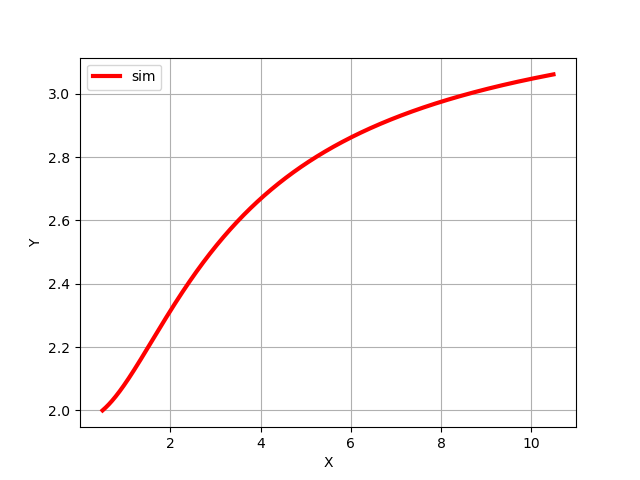
\includegraphics[width=0.75\columnwidth]{figures/Figure_1.png}
\end{figure}
\end{document}


